
\documentclass[11pt,paper=a4,answers]{exam}
\usepackage{graphicx,lastpage}
\usepackage{upgreek}
\usepackage{censor}
\usepackage{tabularx}
\usepackage{xcolor}
\usepackage{amsmath}
%\usepackage{cleveref}
%\usepackage{tabularx,pbox}
\usepackage[nopar]{lipsum}
\usepackage{longtable}
\usepackage{multirow}
\usepackage[inline]{enumitem}
\usepackage{float}
\usepackage{tikz}
\usepackage{amssymb}
\usepackage{pdfrender}
\usepackage{booktabs}
\usepackage{dcolumn}
\usepackage{colortbl}
\newcolumntype{C}{>{\centering\arraybackslash}p{2.5cm}}% for convenience you can also define a new column type

\renewcommand*{\arraystretch}{1.2}%... and increase the row height

\begin{document}
	\begin{minipage}{0.15\linewidth}%
		\flushleft
		
\includegraphics[width=0.85\textwidth]{iare.png}\end{minipage}
	%% \thispagestyle{empty}
	\begin{minipage}[r]{0.85\textwidth}%
		\noindent
		\begin{center}	
			\textcolor{blue}{\Large \bfseries INSTITUTE OF AERONAUTICAL ENGINEERING}\\
			%\hspace*{5.2cm} 
			\textcolor{blue}{\Large (Autonomous)} \\
			%\hspace*{4.7cm}
			\small Dundigal, Hyderabad - 500 043 \\  [3pt] 
		
			\vspace{5pt}
			\large \bfseries AERONAUTICAL ENGINEERING \\\vspace{5pt}
			
			\textcolor{red}{\large \bfseries QUESTION BANK} \\\vspace{3pt}
		\end{center}
	\end{minipage}
	\vspace{0.5cm}
	\par
\newcolumntype{C}[1]{>{\centering\arraybackslash}p{#1}}
\newcolumntype{R}[1]{>{\raggedright\arraybackslash}p{#1}}
\renewcommand{\arraystretch}{1.2}
\vspace{-0.5cm}
\begin{flushleft}
	\begin{longtable}{|R{3.5cm}|R{2.2cm}|R{2.2cm}|C{2.2cm}|C{2.2cm}|C{2.2cm}|}
		\hline
	Course Title                      & \multicolumn{5}{l|}{ \textbf{AEROSPACE STRUCTURAL DYNAMICS}}                                                                  \\ \hline
	Course Code                       & \multicolumn{5}{l|}{AAEC35}                                                                              \\ \hline
	Program                           & \multicolumn{5}{l|}{B.Tech}                                                                              \\ \hline
	Semester                          & VII                         & \multicolumn{4}{l|}{AE}                                                   \\ \hline
	Course Type                       & Core                     & \multicolumn{4}{l|}{}                                                     \\ \hline
	Regulation                        & IARE                   & \multicolumn{4}{l|}{UG20}                                                     \\ \hline
	\multirow{3}{*}{Course Structure} & \multicolumn{3}{c|}{Theory}                                             & \multicolumn{2}{c|}{Practical} \\ \cline{2-6} 
	& \multicolumn{1}{c|}{Lecture} & \multicolumn{1}{c|}{Tutorials} & Credits & Laboratory      & Credits      \\ \cline{2-6} 
	& \multicolumn{1}{c|}{3}       & 1                              & 4       & -               & -            \\ \hline
	Course Coordinator                 & \multicolumn{5}{l|}{Mr. K Arun Kumar, Assistant Professor}                                          \\ \hline                                     
	\end{longtable}
\end{flushleft}
\vspace{-1cm}
%\textcolor{blue}{\large \bfseries COURSE OBJECTIVES:}
\textcolor{blue}{\large \bfseries COURSE OBJECTIVES:}\\
%\vspace{-0.3cm}		
\textbf{The students will try to:}
\vspace{-0.25cm}
\newcolumntype{C}[1]{>{\centering\arraybackslash}p{#1}}
\newcolumntype{R}[1]{>{\raggedright\arraybackslash}p{#1}}
\renewcommand{\arraystretch}{1.2}
\begin{flushleft}	
	\begin{longtable}{|C{1.5cm}|R{15cm}|}
		\hline
		I & Formulate mathematical models of problems in vibrations using Newton’s second law or energy principles.\tabularnewline
		\hline
		II &Determine a complete solution to the modelled mechanical vibration problems.\tabularnewline
		\hline
		III &    design a mechanical system that has desirable vibrational behavior.\tabularnewline
		\hline	
		IV & Assess the underlying assumptions in the aeroelastic analysis of fixed wing and rotary
		wing aerospace vehicles/systems.\tabularnewline
		\hline
	\end{longtable}
\end{flushleft}
\textcolor{blue}{\large \bfseries COURSE OUTCOMES:}\\
%\vspace{-0.3cm}	
\textbf{After successful completion of the course, students should be able to:}\\
\renewcommand{\arraystretch}{1.1}\vspace{-0.75cm}
\begin{flushleft}
	\begin{longtable}{|C{1.5cm}|R{12.5cm}|C{2cm}|}
		\hline
		CO 1 &	\textbf{Apply} \textcolor{blue}{ principles of mechanical vibrations such as Newton’s second law, and
			the principle of conservation of energy to the mathematical models  } \textcolor{red}{for obtaining
			their governing equations of motion.}&Apply\tabularnewline
		\hline
		CO 2&	\textbf{Analyze} \textcolor{blue}{   the mathematical modeling of the two degrees of
			freedom systems} \textcolor{red}{ for determining the frequency of the spring-mass system.}&	Analyze\tabularnewline
		\hline
		CO 3&	\textbf{Solve} \textcolor{blue}{ the natural frequencies and mode shapes of a multi
			degree of freedom system } \textcolor{red}{for the numerical solution of distributed parameter systems}&	Apply\tabularnewline
		\hline 
		
		CO 4&	\textbf{Apply} \textcolor{blue}{  theoretical and numerical procedures } \textcolor{red}{for predicting the dynamic response of  continuous structural systems under the most diverse loading conditions}.	&Apply\tabularnewline
		\hline		
		CO 5&\textbf{Formulate } \textcolor{blue}{ the static aeroelasticity problems such as typical section and wing divergence
			problems; }\textcolor{red}{ for their selection in real world
			applications.}	&	Apply\tabularnewline
		
		
		\hline
	\end{longtable}
\end{flushleft}
\vspace{-0.5cm}
\flushleft\textbf{\textcolor{blue}{\large QUESTION BANK:}}\\
\vspace{-1cm}
\textbf{\large }
	\begin{flushleft}
		\begin{longtable}{|>{\centering\arraybackslash}p{0.8cm}  | >{\raggedright\arraybackslash}p{6.5cm}  | c | >{\raggedright\arraybackslash}p{5cm} |>{\centering\arraybackslash}p{1cm}|} 
			\hline
			\textbf{Q.No}&	\textbf{QUESTION}&\textbf{Taxonomy}&	\textbf{How does this subsume the level}&	\textbf{CO's} \\
			\hline 
			\rowcolor{blue!35}\multicolumn{5}{|c|}{\textbf{MODULE I}}\\
			\hline 
		\rowcolor{yellow!35}\multicolumn{5}{|c|}{\textbf{SINGLE-DEGREE-OF-FREEDOM LINEAR SYSTEMS}}\\
		\hline 	
			\multicolumn{5}{| c |}{\textcolor{red}{\textbf{PART A-PROBLEM SOLVING AND CRITICAL THINKING QUESTIONS}}}\\
		\hline
		1&	A 2 kg block is supported as shown by a spring of constant k = 400 N/m, which can act in
		tension or compression. The block is in its equilibrium position when it is struck from below
		by a hammer, which imparts to the block an upward velocity of 2.5 m/s. Determine i) the
		time required for the block to move 100 mm upward, ii) the corresponding velocity and
		acceleration of the block &	Apply&	The learner will try to \textbf{recall} the function of spring-mass and then \textbf{explain} simplfy the frequency&	CO 1\\
		\hline 
		2&	A block of mass 0.10kg is suspended from a spring having a stiffness of 25N/m. the
		block is displaced downwards from the equilibrium position through a distance of
		2cm and released with an upward velocity of 3cm/sec. Determine
		(i) Natural Frequency (ii) Period of Oscillation (iii) Maximum Velocity
		(iv) Maximum Acceleration (v) Phase angle &	Apply&	The learner will try to \textbf{recall} damped and undamped frequency, Apply it in determining impulse&	CO 1\\
		\hline 
		3& Find the total response of a single degree of freedom system with mass= 10 kg, damping coefficient c= 20 N-s/m, Stiffness= 4000N/m, $ x_{0}= 0.001 m $ and $ \dot{x} = 0 $ under an external force $F(t)=F_{0}\cos \omega t$ acts on a system with  $F_{0}=100N$ and $\omega=10 rad/s$	&		Apply&	The learner will try to \textbf{recall} operation principle response of single degree of freedom.&	CO 1\\
		\hline 
		4& A 3-kg slender rod is suspended from a steel wire which is known to
		have a torsional spring constant K = 2 25 . N m/rad. If the rod is rotated
		through 180° about the vertical and released, determine (a) the period of
		oscillation, (b) the maximum velocity of end A of the rod
		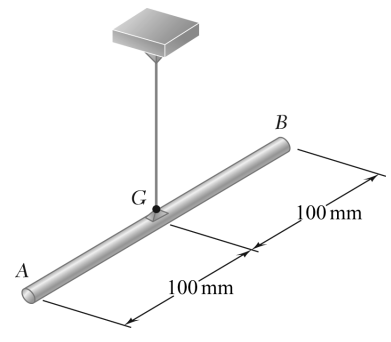
\includegraphics[scale=0.5]{1.png}	&	Apply&	The learner will try to \textbf{recall} the concept beams&	CO 1\\
		\hline 
		5& For a damped system, m, c, and k are known to be m = 1 kg, c = 2 kg/s, k = 10
		N/m. Calculate the value of $\zeta$ and $\omega$n. Is the system overdamped, underdamped, or
		critically damped?	&	Apply&	The learner will try to \textbf{recall} the concept of response of single degree of freedom.&	CO 1\\
		\hline 
		6& Determine the Fourier series for the rectangular wave illustrated in Figure
		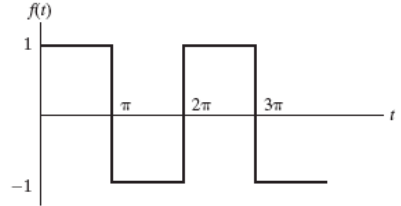
\includegraphics[scale=0.5]{2.png}	&	Apply&	The learner will try to \textbf{recall} the response of single degree of freedom.&	CO 1\\
		\hline 
		7& Determine the Fourier series representation of the sawtooth curve illustrated in Figure
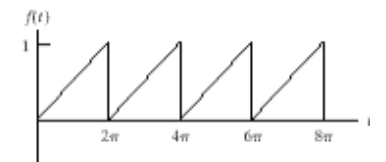
\includegraphics[scale=0.5]{3.png}
	&	Apply&	The learner will try to \textbf{recall} the concepts of frequency and time period &	CO 1\\
		\hline 
		8& Solve the following system for the response x(t) using Laplace transforms:
		100$\ddot{t}$ + 2000x(t) = 50$\delta$(t)
		where the units are in Newtons and the initial conditions are both zero.
&	Apply&	The learner will try to \textbf{recall} the concept beams&	CO 1\\
		\hline 
		9& Investigate the terms involved in the equations of motion of SDOF as given by $\ddot{x}+3\dot{x}+12x=10\sin \omega t$
&	Apply&	The learner will try to \textbf{recall} the concepts of frequency  &	CO 1\\
		\hline
		10 & In a single degree damped vibrating  system mass of 8kg makes 30 oscillations in 18 seconds. The amplitude decreases to 0.35 of the initial value after 5 oscillations. Determine the stifness of the spring, damping factor $\zeta$ and c

&	Apply&	The learner will try to \textbf{recall} the concept of undamped frequency and critical damping&	CO 1\\
		\hline 	
		11 &	A spring-mass system, k1 and m, has a natural frequency of f1. If a second spring k2 is added in
		series with the first spring, the natural frequency is lowered to 1/2
		f1. Determine k2 in terms of k1.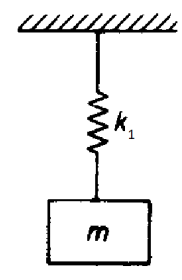
\includegraphics[scale=0.5]{90.png}&	Apply&	The learner will try to \textbf{recall} the concept of undamped frequency and critical damping&	CO 1\\
		\hline 	
			
		\multicolumn{5}{| c |}{\textcolor{red}{\textbf{PART-B LONG ANSWER QUESTIONS}}}\\
		\hline
		1& Dervie the equation of motion for free vibration of an undamped system using Newton's second law of motion.	&	Apply&	The learner will able to understand the concepts of free-undamped vibration.&	CO 1\\
		\hline 
		2& Derive the transfer function of a viscously damped single-degree-of-freedom system subjected to
		external force f(t) as shown in Fig. 
		
		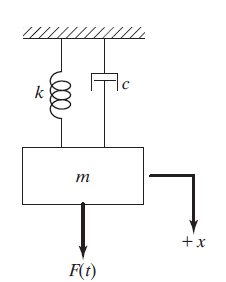
\includegraphics[scale=0.6]{4.png} &	Apply&	The learner will able to understand the concepts of undamped system under harmonic force.&	CO 1\\
		\hline 
		
		3&	Discuss force-displacement relation for linearly elastic and inelastic systems&	Apply&	The learner will able to understand the concepts of damped system under harmonic force.&	CO 1\\
		\hline 
		4&Derive expression for response of a SDOF system subjected to damped free vibration.
		Draw the plot showing response of the structure to damped free vibration explaining
		salient features involved. &		Apply&	The learner will try to \textbf{recall} operation principle response of single degree of freedom.&	CO 1\\
		\hline 
		5&	Dervie the equation of motion of a spring-mass system in vertical position.	&	Apply&	The learner will able to understand the concepts of free-undamped vibration.&	CO 1\\
		\hline 
		6& A harmonic motion is given by $x(t)=10 \sin (30t-\dfrac{\pi}{3})$ mm where tis in seconds and phase angle in radians. Find frequency and period of motion ii) Maximum displacement velocity and acceleration
 &	Apply&	The learner will try to understand the concept of impact excitation. &	CO 1\\
		\hline 
		7&	Discuss the response to an impulse excitation of a single DOF vibrating body.&	Apply&	The learner will try to understand the concept of impulsive excitation.&	CO 1\\
		\hline 
		8& Derive the relation between logarithmic decrement and damping ratio. How is it useful
		in finding damping of a system?	 	&	Apply&	The learner will try to \textbf{recall} the concepts under a periodic force of irregular form.  &	CO 1\\
		\hline 
		9&Summarize the concepts of i) damping ratio  and Critically damping constant  and describe how damped systems are classified based on ddaamping ratio	&	Apply&	The learner will able to understand the concepts of damped system under harmonic force.&	CO 1\\
		\hline 
		10& Dervie the equation of motion for free vibration of an undamped system using Principle of conservation of energy.	&	Apply&	The learner will able to understand the concepts of free-undamped vibration.&	CO 1\\
		\hline   
	11& A periodic motion observed  on the oscilloscope is illustrated in the figure Represent his motion by harmonic series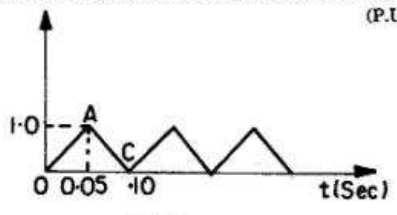
\includegraphics[scale=0.5]{5.png}	&	Apply&	The learner will able to understand the concepts of free-undamped vibration.&	CO 1\\
\hline 
12& What are the three elementary parts of a vibrating system? &	Apply&	The learner will able to understand the concepts of undamped system under harmonic force.&	CO 1\\
\hline 

13&	Consider a spring-mass system with k=4000N/m and m=10kg, with and subject to a harmonic
force $F(t)=400\cos 10t$ Find and plot the total response of the system under the following
initial conditions:
i) $x_{0}=0.1m, \dot{x_{0}}=0m/s$
ii) $x_{0}=0m, \dot{x_{0}}=10m/s$
&	Apply&	The learner will able to understand the concepts of damped system under harmonic force.&	CO 1\\
\hline 
14&List four differences between the free vibrations of an underdamped system and
a system with Coulomb damping. &		Apply&	The learner will try to \textbf{recall} operation principle response of single degree of freedom.&	CO 1\\
\hline 
15&	Describe in detail the following terminologies w.r.t harmonic analysis. i) Cycle ii) Amplitude iii) Period of oscillation iv) Frequency of oscillation v) Phase angle vi) Natural frequency	&	Apply&	The learner will able to understand the concepts of free-undamped vibration.&	CO 1\\
\hline 
16& Write a  note on number of number of degrees of a vibrating system and illustrate three examples of single-degree-of-freedom systems, two degree-of-freedom systems and three -degree-of-freedom systems..
&	Apply&	The learner will try to understand the concept of impact excitation. &	CO 1\\
\hline 
17&Interpret the following concepts with an example:

i) Free and Forced Vibration 

ii) Undamped and Damped Vibration 

iii) Linear and Nonlinear Vibration
iv)Deterministic and Random vibration&	Apply&	The learner will try to understand the concept of impulsive excitation.&	CO 1\\
\hline 
18&  	What is the difference between a discrete and a continuous system? How are the amplitude, frequency, and phase of a steady-state vibration related to those
of the applied harmonic force for an undamped system?	&	Apply&	The learner will try to \textbf{recall} the concepts under a periodic force of irregular form.  &	CO 1\\
\hline 
19&Find the equation of motion for the system shown in Figure when i) $\epsilon=0.3 $	ii) $\epsilon=0.2 $ iii) $\epsilon=2.0$, if the mass m is displaced by a distance of 3cm and released. 

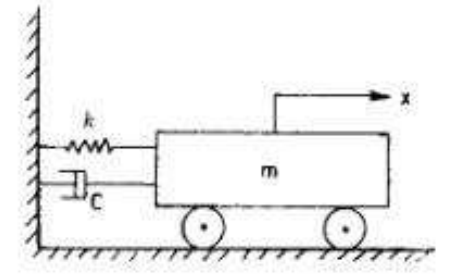
\includegraphics[scale=0.5]{7.png} &	Apply&	The learner will able to understand the concepts of damped system under harmonic force.&	CO 1\\
\hline 
20& Explain in detail variouus types of damping used in mechanical systems and write the displacement equations	&	Apply&	The learner will able to understand the concepts of free-undamped vibration.&	CO 1\\
\hline 
	\multicolumn{5}{| c |}{\textcolor{red}{ \textbf{PART-C SHORT ANSWER QUESTIONS}}}\\
	\hline 
	1&	What is Vibration? &	Understand&	The learner will try to \textbf{recall} the definition of vibration&	CO 1\\
	\hline 
	2&	Define natural frequency. Why is it important ?  &	Remember&	&	CO 1\\
	\hline 
	3&	Define Free vibrations.&	Remember&	–&	CO 1\\
	\hline 
	4&	Define forced vibrations.  &	Remember&	–&	CO 1\\
	\hline 
	5&	Define Resonance with example.&	Understand&	The learner will try to recall basics of vibrations. &	CO 1\\
	\hline 
	6&	Define damped vibrations. &	Understand&	The learner will try to understand the difference of damped and undamped.&	CO 1\\
	\hline 
7&State the parameters corresponding to m, c, k, and x for a torsional system. &	Remember&	&	CO 1\\
\hline 
8& What effect does a decrease in mass have on the frequency of a system? &	Remember&	&	CO 1\\
\hline 
9& What effect does a decrease in the stiffness of the system have on the natural period? &	Remember&	&	CO 1\\
\hline 
10& Why does the amplitude of free vibration gradually diminish in practical systems? &	Remember&	&	CO 1\\
\hline 
11&Can the energy method be used to find the differential equation of motion of all singledegree-
of-freedom systems? &	Remember&	&	CO 1\\
\hline 
12& What assumptions are made in finding the natural frequency of a single-degree-offreedom
system using the energy method? &	Remember&	&	CO 1\\
\hline 
13& What methods are available for solving the governing equations of a vibration problem? &	Remember&	&	CO 1\\
\hline 
14& How do you connect several springs to increase the overall stiffness? &	Remember&	&	CO 1\\
\hline 
15& Define spring stiffness and damping constant. &	Remember&	&	CO 1\\
\hline 
16& What are the common types of damping? &	Remember&	&	CO 1\\
\hline 
17& State three different ways of expressing a periodic function in terms of its harmonics &	Remember&	&	CO 1\\
\hline 
18&What will be the frequency of the applied force with respect to the natural frequency of
the system if the magnification factor is less than unity? &	Remember&	&	CO 1\\
\hline 
19& What happens to the response of an undamped system at resonance? &	Remember&	&	CO 1\\
\hline 
20 & What is the difference between the peak amplitude and the resonant amplitude? &	Remember&	&	CO 1\\
\hline 
	\hline 	
			\rowcolor{blue!35}\multicolumn{5}{| c |}{\textbf{MODULE II}}\\
		\hline 
	\rowcolor{yellow!35}\multicolumn{5}{| c |}{ \textbf{TWO-DEGREE-OF-FREEDOM SYSTEMS}}\\
	\hline 
	\multicolumn{5}{| c |}{\textcolor{red}{\textbf{PART-A PROBLEM SOLVING AND CRITICAL THINKING QUESTIONS}}}\\
	\hline
	1&	Find the natural frequencies and mode shapes of a spring-mass system, shown in Figure, which is constrained to move in the vertical direction only. Take n=1
	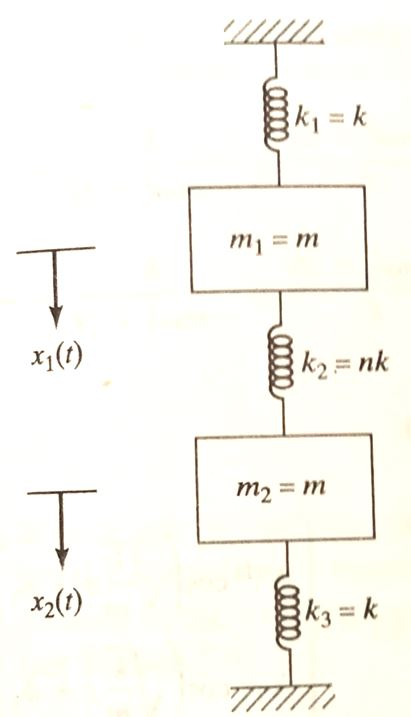
\includegraphics[scale=0.3]{1.jpg}
&	Apply&	The learner will try to \textbf{recall} natural frequencies of spring-mass system.&	CO 2\\
	\hline 
	2&	Find the free vibration response of the system shown in figure with $k_1=30, k_2=5, k_3=0, m_1=10, m_2=1, and c_1=c_2=c_3=0 $ for the initial conditions $ x_1(0)=1, x_1(0)/t=x_2(0)=x_2(0)/t=0 $. 
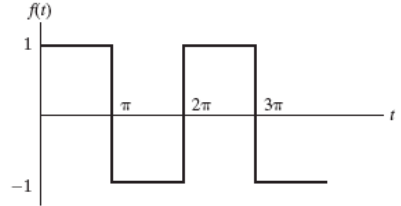
\includegraphics[scale=0.4]{2.jpg}
&	Apply&	The learner will try to \textbf{recall} the free vibration response of two DOF.&	CO 2\\
	\hline 
	3&	Find the natural frequencies and mode shapes for the torsional system shown in figure for $ J_1=J_0=2J_0, $ and $ k_{t1}=k_{t2}=k_t. $ 
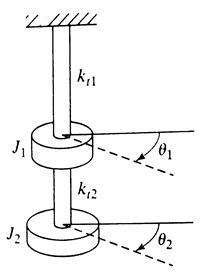
\includegraphics[scale=0.5]{3.jpg}
&	Apply&	The learner will try to \textbf{recall} the natural frequencies of a torsional system. &	CO 2\\
	\hline 
	4&	Consider the two-degree-of-freedom system described by
	\newline
$\begin{Bmatrix}
	1& 0\\
	0& 1
\end{Bmatrix}	\begin{Bmatrix}\ddot{x_{1}}\\\ddot{x_{2}}\end{Bmatrix}$
+
$\begin{Bmatrix}
		0& 0\\
	0 &c
\end{Bmatrix}	\begin{Bmatrix}\dot{x_{1}}\\\dot{x_{2}}\end{Bmatrix}
\newline	+
\begin{Bmatrix}	2& -1\\
	-1& 2\end{Bmatrix}	\begin{Bmatrix}x_{1}\\x_{2}\end{Bmatrix}=\begin{Bmatrix}f_{0}\sin \omega t\\0\end{Bmatrix}$

	and calculate the transfer function |X/F| as a function of the damping parameter c.

&	Apply&	The learner will try to \textbf{recall} the mode shape of a torsional system. &	CO 2\\
	\hline 
	5&	Formulate the equation of motion for two degree of freedom system for damped free
	vibration.
 &	Apply&	The learner will try to \textbf{recall} the response under impulse using Laplace transform method.&	CO 2\\
	\hline 
	6&	Find the natural frequencies of the system shown in figure, with $m_1=m, m_2=2m, k_1=k, $ and $ k_2=2k$. Determine the response of the system when k=1000 N/m, m=20kg, and the initial values of the displacement of the masses $m_1=1 $and $m_2=-1$ respectively.
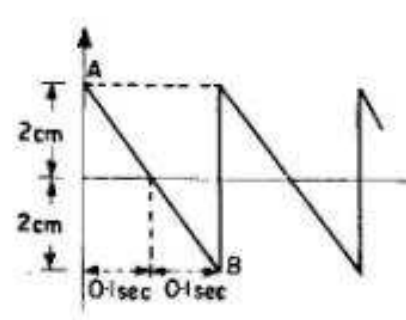
\includegraphics[scale=0.3]{6.jpg}
&	Apply&	The learner will try to \textbf{recall} the response of spring-mass system&	CO 2\\
	\hline 
7& Find the free vibration response of the spring-mass-damper system shown in figure with $k_1=40, k_2=10, k_3=2, m_1=9, m_2=12, and c_1=1, c_2=c_3=0 $ for the initial conditions $ x_1(0)=1.5, x_1(0)/t=x_2(0)=x_2(0)/t=0.5 $. 
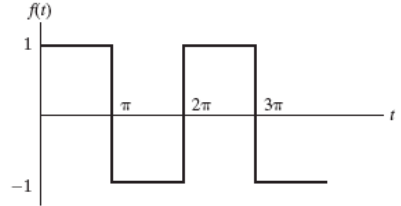
\includegraphics[scale=0.4]{2.jpg}
&	Apply&	The learner will try to \textbf{recall} the free vibration response of two DOF.&	CO 2\\
	\hline 
	8& The stiffness matrix and mass matrix of a two degree fredom system are given by K=$\begin{Bmatrix}
		4&2\\2&4
	\end{Bmatrix}$ and m= $\begin{Bmatrix}
	1&0\\0&1
\end{Bmatrix}$ Determine the natural frequencies and modes of vibration normalized w.r.t matrix such that $x^{T}mx=1$
	&	Apply&	The learner will try to apply the concepts of two DOF for practicle problems. &	CO 2\\
		\hline 
9&	Determine the transfer function for the 20 kg block of the system in Figure 6.10 due to a
force applied to the 20 kg block.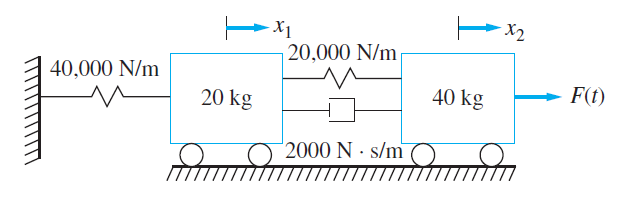
\includegraphics[scale=0.3]{6.10.png}
&	Apply&	The learner will try to \textbf{recall} the response of spring-mass system&	CO 2\\
	\hline 
10&	Find the natural frequencies of a spring-mass system, shown in Figure, for $k_1=300 N/m, k_2=500 N/m, k_3=200 N/m, m_1=2kg $ and $m_2=1kg$.
	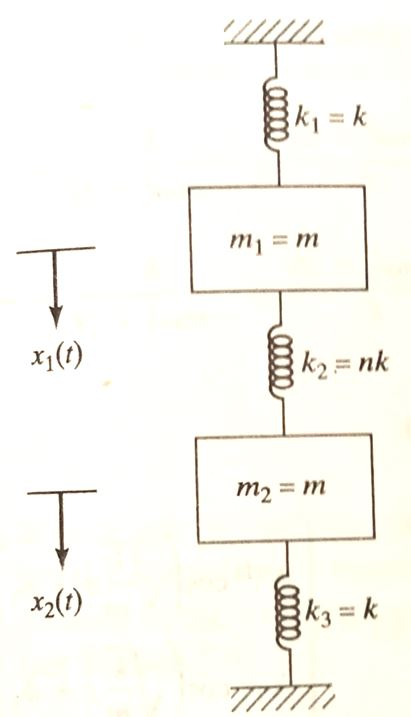
\includegraphics[scale=0.4]{1.jpg}
&	Apply&	The learner will try to \textbf{recall} natural frequencies of spring-mass system.&	CO 2\\
	\hline 
		\multicolumn{5}{| c |}{\textcolor{red}{ \textbf{PART-B LONG ANSWER QUESTIONS}}}\\
		\hline
		1&	Derive the equation of motion for forced vibration of spring-mass-damping system.
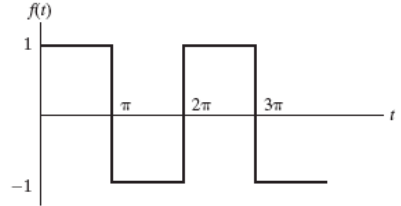
\includegraphics[scale=0.4]{2.jpg}
&	Apply&	The learner will try to \textbf{recall} natural frequencies of spring-mass system.&	CO 2\\
		\hline 
		2&	Derive the frequency equation for free vibration analysis of an undamped system.&	Apply&	The learner will able to \textbf{recall} the experssion of free vibration analysis of an undamped system.&	CO 2\\
		\hline 
		3&	Derive equation of motion of multi degree freedom systems by
		(i) Newton’s equation of motion
		(ii) Mass spring damper system
		(iii) Dynamic equilibrium &	Apply&	The learner will able to \textbf{recall} the experssion of free vibration analysis of an undamped system.&	CO 2\\
		\hline 
		4&	Describe the experssions for the free vibrational analysis for torsional system.&	Understand&	The learner will try to \textbf{recall} the free vibrational analysis for torsional system. &	CO 2\\
		\hline 		
5	&Derive the equation of motion of the system shown in Figure . Assume that the initial tension ‘T’
	in the string is too large and remains constants for small amplitudes. Determine the natural
	frequencies, the ratio of amplitudes and locate the nodes for each mode of vibrations when m1 = m2
	= m and l1= l2 = l3 = l.	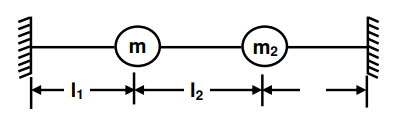
\includegraphics[scale=0.7]{80.png}&	Apply&	The learner will try to \textbf{recall} natural frequencies of spring-mass system.&	CO 2\\
		\hline 
		6& Derive the equation of motion for two degree of freedom under external forces.	&	Apply&	The learner will try to \textbf{recall} the two degree of freedom under external forces.&	CO 2\\
		\hline 
		7& What is meant by static and dynamic coupling? How can you eliminate coupling of the
		equations of motion
	&	Apply&	The learner will try to apply the concepts of two DOF for practicle problems. &	CO 2\\
		\hline 
8&	The transfer function for one generalized coordinate of a two degree-of-freedom
system is $G(s)=\dfrac{1}{s^{4}+3s^{2}+2}$

i) Calculate G(3i).

ii) What are the natural frequencies of the system?

iii) If this system were excited by a force equal to 5 sin3t, what is the
steady-state response of the generalized coordinate?

&	Apply&	The learner will try to recall the concept of natural frequency and understand the equations of motion for MDOF and determine the the transfer function for different mechanical systems &	CO 2\\
	\hline 
9& Derive the frequency experssion for un-restrained systems with diagram.&	Apply&	The learner will try to recall the concept of natural frequency and understand the equations of motion for MDOF and determine the the natural frequency for different mechanical systems &	CO 2\\
	\hline 
10 & Find the free-vibration solution of the unrestrained system shown in figure for the following
data: $k= 200 N/m, m_1= 1 kg, m_2= 2 kg, and c_1=1, c_2=c_3=0 $ for the initial conditions $ x_1(0)= 0.1 m, x_2(0)/t=x_2(0)/t=0. $. 
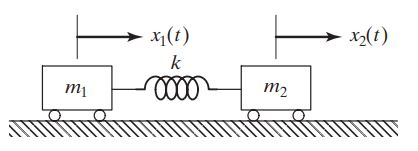
\includegraphics[scale=0.4]{8.jpg}
&	Apply&	The learner will try to recall the concept of natural frequency and understand the equations of motion for MDOF and determine the the natural frequency for different mechanical systems &	CO 2\\
	\hline 
11 & The two degree-of-freedom system shown in Figure 6.34 is subject to the periodic force
shown. Determine the steady-state response of the system.
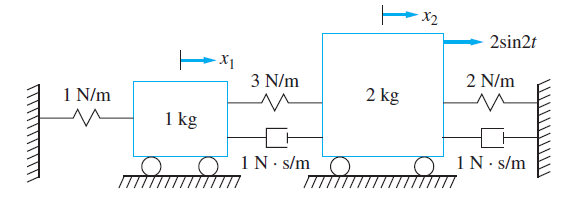
\includegraphics[scale=0.4]{6.34.png}
&	Apply&	The learner will try to recall the concept of natural frequency and understand the equations of motion for MDOF and determine the the natural frequency for different mechanical systems &	CO 2\\
\hline 
12 & Determine the natural frequencies and mode shapes for the two degree-of-freedom system
shown in Figure 6.33.
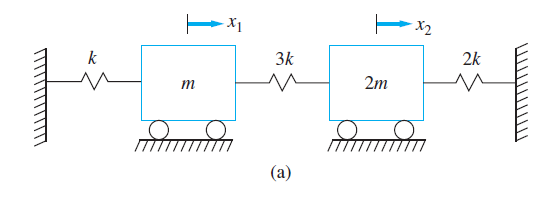
\includegraphics[scale=0.4]{6.33.png}
&	Apply&	The learner will try to recall the concept of natural frequency and understand the equations of motion for MDOF and determine the the natural frequency for different mechanical systems &	CO 2\\
\hline
13 & The system of Figure 6.9 is at rest in equilibrium when a unit impulse is applied to the 2 kg
block. Determine the resulting response of the 1 kg block.
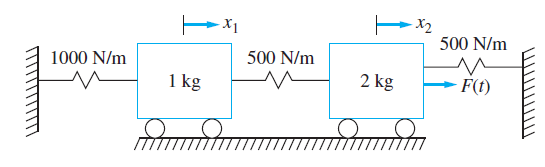
\includegraphics[scale=0.4]{6.9.png}
&	Apply&	The learner will try to recall the concept of natural frequency and understand the equations of motion for MDOF and determine the the natural frequency for different mechanical systems &	CO 2\\
\hline 
14 & Determine the response of the system of Figure 6.5 when using $x_{1}$ and $x_{2}$ as generalized
coordinates when $\dot{x_{2}}-2m/s$ and all other initial conditions are zero.
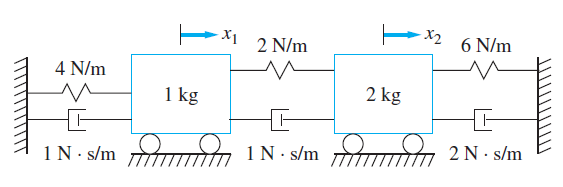
\includegraphics[scale=0.4]{6.5.png}
&	Apply&	The learner will try to recall the concept of natural frequency and understand the equations of motion for MDOF and determine the the natural frequency for different mechanical systems &	CO 2\\
\hline
15& Consider the two degree-of-freedom system of Figure 6.6. Determine the steady-state
response of the system.
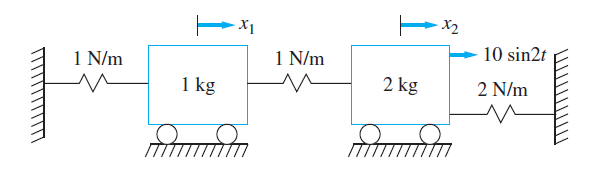
\includegraphics[scale=0.4]{6.6.png}
&	Apply&	The learner will try to recall the concept of natural frequency and understand the equations of motion for MDOF and determine the the natural frequency for different mechanical systems &	CO 2\\
\hline 
16 & Find the steady-state response for the system of Figure 6.7.
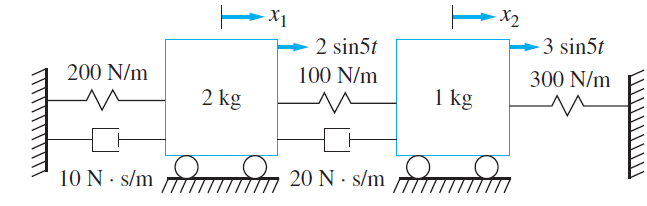
\includegraphics[scale=0.4]{6.7.png}
&	Apply&	The learner will try to recall the concept of natural frequency and understand the equations of motion for MDOF and determine the the natural frequency for different mechanical systems &	CO 2\\
\hline
17 & Derive the differential equations governing the damped two degree-of-freedom
system shown in Figure P6.6 using x1 and x2 as generalized coordinates
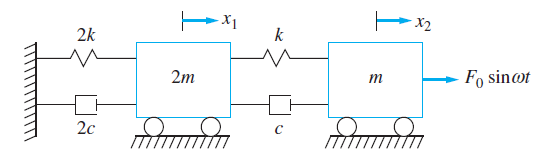
\includegraphics[scale=0.4]{5p6.6.png}
&	Apply&	The learner will try to recall the concept of natural frequency and understand the equations of motion for MDOF and determine the the natural frequency for different mechanical systems &	CO 2\\
\hline 

			\multicolumn{5}{| c |}{\textcolor{red}{ \textbf{PART-C SHORT ANSWER QUESTIONS}}}\\
		\hline 
		1&	Define the two DOF with suitable figure. &	Remember&	–&	CO 2\\
		\hline 
		2&	Define semidefinite systems with example.&	Remember&	–&	CO 2\\
		\hline 
		3&	What  are static couplings?&	Remember&	–&	CO 2\\
		\hline 
		4&	Define generlized coordinates in vibration.&	Remember&	–&	CO 2\\
		\hline 
		5&	Define Principal coordinates.&	Remember&	–&	CO 2\\
		\hline 
		6&	What  are dynamic couplings?&	Remember&	–&	CO 2\\
		\hline 
		7&	Write a short note on torsional vibration for two DOF with example.&	Remember&	–&	CO 2\\
		\hline 
		8& Define elasticity coupling.&	Remember&	–&	CO 2\\
		\hline 
		
9&	Define the sinusoidal transfer function.&	Remember&	–&	CO 2\\
	\hline 
10& Write the differential equations for the principal coordinates of free undamped
	vibrations of a two degree-of-freedom system with natural frequencies $\omega$1 and $\omega$2.&	Remember&	–&	CO 2\\
	\hline 
11& A two degree-of-freedom system has a mode with a modal fraction equal to
	zero. What does this imply?&	Remember&	–&	CO 2\\
	\hline 
12& A two degree-of-freedom system has a mode with a modal fraction equal to one.
	What does this imply?&	Remember&	–&	CO 2\\
	\hline 
13& How many nodes are there for the mode corresponding to the lowest natural
	frequency of a two degree-of-freedom system?&	Remember&	–&	CO 2\\
	\hline 
		\rowcolor{blue!35}\multicolumn{5}{| c |}{\textbf{MODULE III}}\\
	\hline 
	\rowcolor{yellow!35}\multicolumn{5}{| c |}{\textbf{MULTI-DEGREE-OF-FREEDOM LINEAR SYSTEMS}}\\
	\hline 
		\multicolumn{5}{| c |}{\textcolor{red}{\textbf{PART A-PROBLEM SOLVING AND CRITICAL THINKING QUESTIONS}}}\\
	\hline
	1&	The vibrations of a cantilever are given by $y=y_{l}(1-\cos \dfrac{\pi x}{2l})$ Calculate the frequency with the following data for the cantilever using Rayleigh method. Modulus of amterial is $2 \times 10^{11}n?m^{2}$
	Second moment of inertia about bending axis is $0.02m^{4}$ $Mass=6 \times 10^{4} kg$ $length=30m$
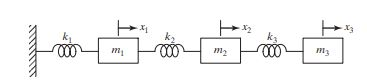
\includegraphics[scale=0.6]{15.jpg}
&	Apply&	The learner will try to \textbf{recall} the concepts of stiffness influence coefficients. &	CO 3\\
	\hline
	2&	Determine the naatural frequency of multidegree of freedom spring mass system shown in figure 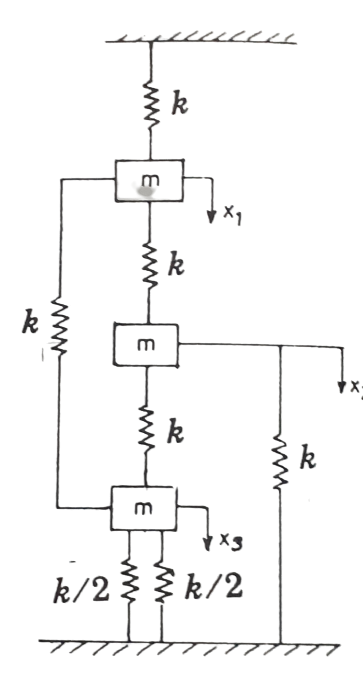
\includegraphics[scale=0.3]{6_3.png}
&	Apply&	The learner will try to \textbf{recall} the concepts of flexibility influence coefficients.&	CO 3\\
	\hline
	3&	A shaft of negligable weight 6cm diasmeter and 5m long is simply supported at the ends and carries four weights 50kg each at equal distance over the length of the shaft. Find the frequency of vibrations using Dunkerly method. Take $E=2 \times 10^{6}kg/cm^{2}$
	
	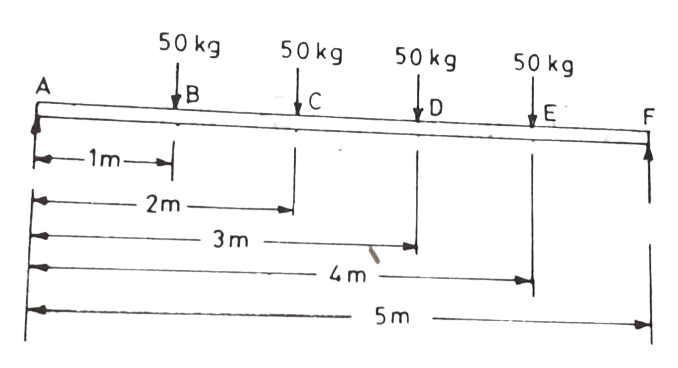
\includegraphics[scale=0.25]{6_9.png}
&	Apply&	The learner will try to \textbf{recall} the concepts of flexibility influence coefficients. &	CO 3\\
	\hline
	4&Find the natural frequency of transverse vibrations for a uniformly distributed system shown in Figure  using Dunkerly method
	
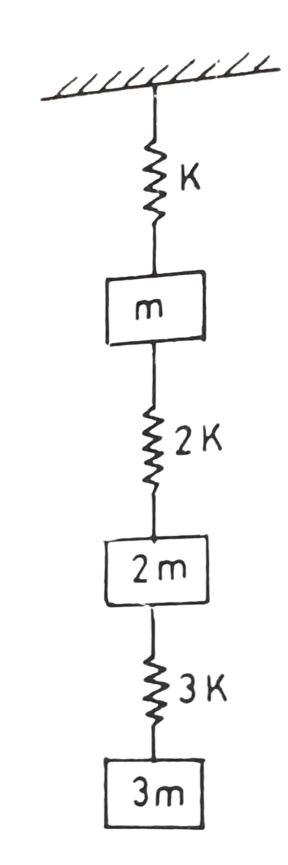
\includegraphics[scale=0.2]{6_10.png}
&	Apply&	The learner will try to \textbf{recall} the concepts of inertia influence coefficients.&	CO 3\\
	\hline
	5&	Find the natural frequency and mode shapes by using influence coefficients for the mechanical system shown in Figure 
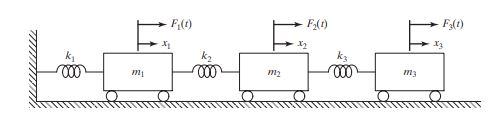
\includegraphics[scale=0.45]{18.jpg}
&	Apply&	The learner will try to \textbf{recall} the working principle and classification of engine cycles and then \textbf{explain} the differences between them and then compare their merits&	CO 4\\
	\hline
6&	Find the natural frequency of vibration for the system shown in figure by Rayleigh method.

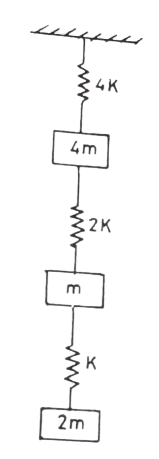
\includegraphics[scale=0.4]{6_15.png}&	Apply&	The learner will try to \textbf{recall} the concept of Mono propellant and Bi propellant and then \textbf{explain}s the advantages over the other&	CO 4\\
	\hline
	7& 
Write equations of motion and determine first mode shape  of the system  given in Figure using eigen values and eigen vectors

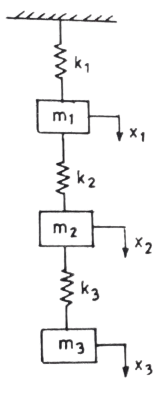
\includegraphics[scale=0.3]{6_16.png}
	&	Apply&	The learner will try to apply the concepts of two DOF for practicle problems. &	CO6\\
		\hline 
8&	
Find the natural frequency of the spring mass system shown in Figure by matrix method

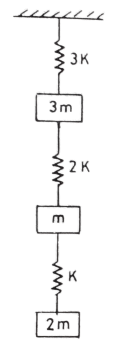
\includegraphics[scale=0.2]{6_17.png}
&	Apply&	The learner will try to \textbf{recall} the natural frequencies of a torsional system. &	CO 4\\
	\hline 
9& A steel shaft of diameter 10cm is carrying three masses 5kg, 7.5kg and 14kg respectively. The distances between the rotors are 0.70m. Determine the natural frequencies of torsional vibrations. The radius of gyrations of three rotors are 0.20, 0.20, 0.40. Take $G=9\times 10^{8}N/m^{2}$

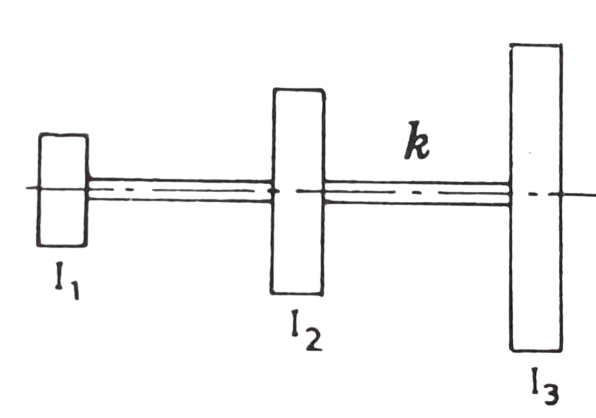
\includegraphics[scale=0.2]{6_12.png}&	Apply&	The learner will try to recall the concept of natural frequency and understand the equations of motion for MDOF and determine the the natural frequency for different mechanical systems 

&	CO 4\\
	\hline 
10 & Find the free-vibration solution of the unrestrained system shown in figure for the following
data: $k= 200 N/m, m_1= 1 kg, m_2= 2 kg, and c_1=1, c_2=c_3=0 $ for the initial conditions $ x_1(0)= 0.1 m, x_2(0)/t=x_2(0)/t=0. $. 

&	Apply&	The learner will try to recall the concept of natural frequency and understand the equations of motion for MDOF and determine the the natural frequency for different mechanical systems &	CO 4\\
	\hline 
	\multicolumn{5}{| c |}{\textcolor{red}{ \textbf{PART-B LONG ANSWER QUESTIONS}}}\\
	\hline
	1&	Discuss the procedure that can be adopted to derive the equation of motion of a multi degree of freedom.&	Understand&	The learner will try to \textbf{recall} concepts of multi degree of freedom. &	CO 3\\
	\hline
	2& Estimate the lowest natural frequency transverse vibration for the system shown in Figure by using Rayleigh method. Take $E-2\times 10^{11}N/m^{2},I=10^{-6}m^{4}, g=10m/s^{2}$
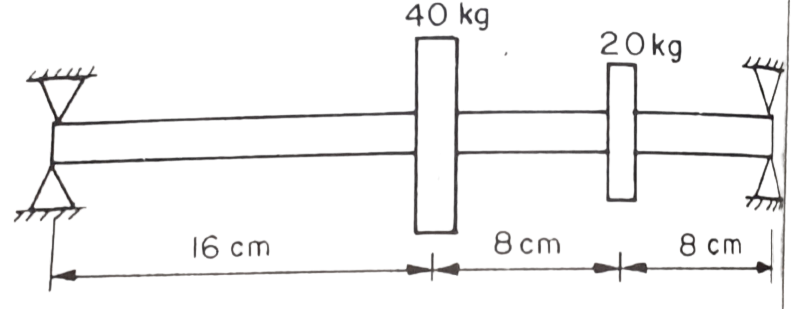
\includegraphics[scale=0.24]{6_11.png}
	&	Apply&	The learner will try to \textbf{recall} concepts of stiffness matrix.&	CO 3\\
	\hline
	3&	Dervie the equation of motion of the spring-mass-damper system shown in the figure.
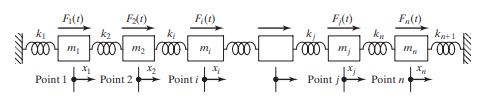
\includegraphics[scale=0.47]{14.jpg}
&	Apply&	The learner will try to understand the derivation of multi DOF.&	CO 4\\
	\hline
	4&	What are the aspects that influence the stiffness coefficients for multi degree vibrating system?&	Apply&	The learner will try to identify the influence factors of stiffness.&	CO 4\\
	\hline
	5&	What are the aspects that influence the flexibility coefficients for multi degree vibrating system?&	Apply&	The learner will try to identify the influence factors of flexibility.&	CO 4\\
	\hline
	6&	An undamped vibration pickup having a natural frequency of 1Hz is used to measure a harmonic vibration of 4Hz. If the amplitude recorded is 0.52mm, what is the correct amplitude?&	Apply&	The learner will try to \textbf{recall} the concept of Mono propellant and Bi propellant and then \textbf{explain}s the advantages over the other&	CO 4\\
	\hline
1&	Find the stiffness influence coefficients of the system shown in the figure.
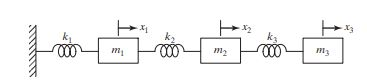
\includegraphics[scale=0.6]{15.jpg}
&	Apply&	The learner will try to \textbf{recall} the concepts of stiffness influence coefficients. &	CO 3\\
\hline
8&	Find the lowest natural frequency of the mechanical system shown in Figure 

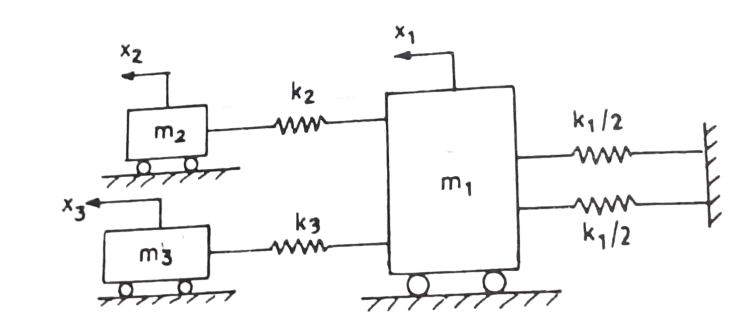
\includegraphics[scale=0.2]{6_14.png}
&	Apply&	The learner will try to \textbf{recall} the natural frequencies of a torsional system. &	CO 4\\
	\hline 
9& Derive the frequency experssion for un-restrained systems with diagram.&	Apply&	The learner will try to recall the concept of natural frequency and understand the equations of motion for MDOF and determine the the natural frequency for different mechanical systems &	CO 4\\
	\hline 
10 & Find the free-vibration solution of the unrestrained system shown in figure for the following
data: $k= 200 N/m, m_1= 1 kg, m_2= 2 kg, and c_1=1, c_2=c_3=0 $ for the initial conditions $ x_1(0)= 0.1 m, x_2(0)/t=x_2(0)/t=0. $. 

&	Apply&	The learner will try to recall the concept of natural frequency and understand the equations of motion for MDOF and determine the the natural frequency for different mechanical systems &	CO 4\\
	\hline 
	11&	Derive the flexibility matrix of the weightless beam shown in Figure. The beam is simply supported at both ends, and the three masses are placed at equal intervals. Assume the beam to be uniform with stiffness EI. 
	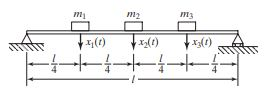
\includegraphics[scale=0.8]{16.jpg}
	&	Apply&	The learner will try to \textbf{recall} the natural frequencies of a torsional system. &	CO 4\\
	\hline
		12&	Find the flexibility coefficients influence coefficients of the system shown in the figure.
		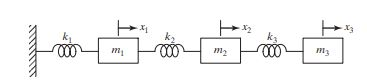
\includegraphics[scale=0.6]{15.jpg}
	&	Apply&	The learner will try to \textbf{recall} the natural frequencies of a torsional system. &	CO 4\\
	\hline
		13&	Explain the coupling of coordinates in MDOF system. How will you obtain the type of coupling present by the help of matrices and energy expressions
	&	Apply&	The learner will try to \textbf{recall} the natural frequencies of a torsional system. &	CO 4\\
	\hline
	14&	Find the equations of motion of a multidegree-of-freedom system in matrix form using
	a. the flexibility matrix and
	b. the stiffness matrix.
	&	Apply&	The learner will try to \textbf{recall} the natural frequencies of a torsional system. &	CO 4\\
	\hline
		15&	Determine the eigenvalues and eigenvectors of the system shown in Fig. 6.29, taking $k_{1}=k_{2}=k_{3}=k_{4}=k$, $m_{1}=2m\,\,m_{2}=3m\,\,m_{3}=5m$
		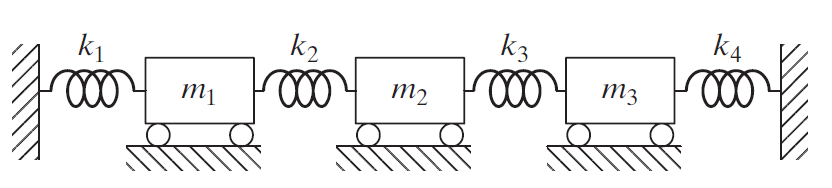
\includegraphics[scale=0.4]{6.29.png}
	&	Apply&	The learner will try to \textbf{recall} the natural frequencies of a torsional system. &	CO 4\\
	\hline
	16&	Three rail bogies are connected by two springs of stiffness $40 \times 10^{6}n/m$ each. The mass of each bogey is $20\times 10^{3} kg$  Determine the frequecies of vibration Neglect wheels and rails
	
	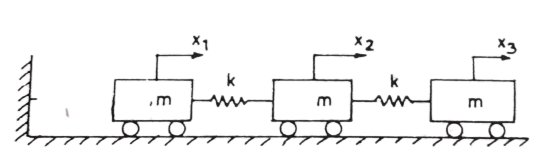
\includegraphics[scale=0.4]{6_18.png}
	&	Apply&	The learner will try to \textbf{recall} the natural frequencies of a torsional system. &	CO 4\\
	\hline

		\multicolumn{5}{| c |}{\textcolor{red}{ \textbf{PART-C SHORT ANSWER QUESTIONS}}}\\
	\hline
	
		1&	Define multi degree of freedom with example.&	Remember&	–&	CO 3\\
	\hline 
	2&Define unrestrained systems.&	Remember&	–&	CO 3\\
	\hline 
	3&	Write short notes on modal analysis.&	Remember&	–&CO 3\\
	\hline 
	4&What is a mode shape?&	Remember&	–&	CO 3\\
	\hline 
	5&	Write the steps to derive the equation of motion of multi DOF system using Newton's second law.&	Remember&	–&	CO 3\\
	\hline 
	6&	What is the need for vibration measuring instruments?&	Remember&	–&CO 3\\
	\hline 
	7&	Draw the sketch of a seismic instrument and label the parts.&	Remember&	–&	CO 3\\
	\hline 

8& State Lagrange s equations.&&	–&	CO 2\\
\hline 
9& What is an eigenvalue problem?&&	–&	CO 2\\
\hline 
10& What is a mode shape? How is it computed?&&	–&	CO 2\\
\hline 
11& How many distinct natural frequencies can exist for an n-degree-of-freedom system?&&	–&	CO 2\\
\hline 
12& What is a dynamical matrix? What is its use?&&	–&	CO 2\\
\hline 
13& How is the frequency equation derived for a multidegree-of-freedom system?&	&–&	CO 2\\
\hline 
14& What is meant by the orthogonality of normal modes? What are orthonormal modal vectors?&&	–&	CO 2\\
\hline 
15& What is a basis in n-dimensional space?&&	–&	CO 2\\
\hline 
16& What is the expansion theorem? What is its importance?&&	–&	CO 2\\
\hline 
17& Explain the modal analysis proceduce.&&	–&	CO 2\\
\hline 
18& What is a rigid-body mode? How is it determined?&&	–&	CO 2\\
\hline 
19& What is a degenerate system?&&	–&	CO 2\\
\hline 
20& How can we find the response of a multidegree-of-freedom system using the first few
modes only?&&	–&	CO 2\\
\hline 
21&Define Rayleigh s dissipation function.&&	–&	CO 2\\
\hline 
22& Define these terms: proportional damping, modal damping ratio, modal participation factor.&&–&	CO 2\\
\hline 
23& When do we get complex eigenvalues?&&	–&	CO 2\\
\hline 
24&What is the difference between generalized coordinates and Cartesian coordinates?&&	–&	CO 2\\
\hline 
		\rowcolor{blue!35}\multicolumn{5}{| c |}{\textbf{MODULE IV}}\\
	\hline 
	\rowcolor{yellow!35}\multicolumn{5}{| c |}{ \textbf{DYNAMICS OF CONTINUOUS ELASTIC BODIES}}\\\hline
		\multicolumn{5}{| c |}{\textcolor{red}{\textbf{PART A- PROBLEM SOLVING AND CRITICAL THINKING QUESTIONS}}}\\
	\hline
	1&	Explain the consequences of misalignment and pre loaded shafts on the performance of the machine assembly with plots.&	Analyze&	The learner will try to \textbf{recall} RCS and payload fraction and \textbf{explain}s its importance and application of RCS&	CO 5\\
	\hline
	2&	Explain the procedure to find out natural frequency of vibrations by Dunker leys method for simple supported beam subjected to three point loads at equidistance along the span&	Analyze&	The learner will try to \textbf{recall} the importance of staging of rocket and then \textbf{explain}s the different mechanism’s that are used for staging of rocket&	CO 5\\
	\hline
	3&	A shaft of negligible weight 6 cm diameter and 5 meters long is simply supported at the ends and carries four weights 50 kg each at equal distance over the length of the shaft as shown in Figure. Find the frequency of vibration by Dunkerley's method.
Take E = 2 x 106 kg / cm2 if the ends of the fixed.
&	Analyze&	The learner will try to \textbf{recall} the importance of staging of rocket and then \textbf{explain} the concept of rocket dispersion &	CO 5\\
	\hline
	4&	What conclusion can be drawn during condition monitoring of mechanical systems using failure mode analysis? and \textbf{explain} the function of gyroscope and accelerometer&	Analyze&		The learner will try to \textbf{recall} the concept of Inertial guidance systems  and \textbf{explain} the working of gyroscope and accelerometer in&	CO 5\\
	\hline
	5&	Explain different types of data acquisition systems with compression to merits and demerits of each other.&	Analyze&	The learner will try to \textbf{recall} the concept of Wing configuration of missile and then \textbf{explain} the concept of wing and canard configuration with a neat sketch&	CO 5\\
	\hline
	6&	Explain signature analysis of a mechanical system subjected to forced vibration.&	Analyze&	The learner will try to \textbf{recall} the importance of staging of rocket and then \textbf{explain}s the advantages of multi-staging over a single stage rocket&	CO 5\\
	\hline
	7&	Root cause analysis is very essential for introducing to implement using fishbone chart. Explain.&	Analyze&	The learner will try to \textbf{recall} the concept of Wing configuration of missile and then \textbf{explain}s the concept of wing and canard configuration with a neat sketch&	CO 5\\
	\hline
8&	Turbo engine connected to a propeller through gears shown in figure. The mass moments of inertia of the flywheel, engine, gear 1, gear 2 and the propeller are 10000, 1500, 200, and 2500 $ (kg-m^2) $ respectively. Find the natural frequencies of the system in torsional vibration. 

&	Apply&	The learner will try to \textbf{recall} the natural frequencies of a torsional system. &	CO 5\\
	\hline 
9& Derive the frequency experssion for un-restrained systems with diagram.&	Apply&	The learner will try to recall the concept of natural frequency and understand the equations of motion for MDOF and determine the the natural frequency for different mechanical systems &	CO 5\\
	\hline 
10 & Find the free-vibration solution of the unrestrained system shown in figure for the following
data: $k= 200 N/m, m_1= 1 kg, m_2= 2 kg, and c_1=1, c_2=c_3=0 $ for the initial conditions $ x_1(0)= 0.1 m, x_2(0)/t=x_2(0)/t=0. $. 

&	Apply&	The learner will try to recall the concept of natural frequency and understand the equations of motion for MDOF and determine the the natural frequency for different mechanical systems &	CO 5\\
	\hline 
	\multicolumn{5}{| c |}{\textcolor{red}{ \textbf{PART-B LONG ANSWER QUESTIONS}}}\\
	\hline
	1&	Explain trending analysis.&	Understand&	The learner will try to \textbf{recall} the concept of Wing configuration of missile and then \textbf{explain} the concept of wing and canard configuration with a neat sketch&	CO 5\\
	\hline
	2&Explain failure node analysis.&	Understand&	The learner will try to \textbf{recall} the concept of wing aerodynamics and then \textbf{explain} the concept of upwash and downwash with neat  sketches&	CO 5\\
	\hline	
	3&	Explain root cause analysis.&	Understand&	The learner will try to \textbf{recall} the concept of guidance systems in rocket and missiles and \textbf{explain} the purpose of using the guidance system&	CO 5\\
	\hline
	4&	Explain signature analysis.&	Understand&	The learner will try to \textbf{recall} the operation of missile and then \textbf{explain} guidance phases of missiles&	CO 5\\
	\hline
	5&	Explain machine monitoring parameters.&	Understand&	The learner will try to \textbf{recall} the concept of guidance systems in rocket and missiles and \textbf{explain} the classification with neat sketches&	CO 5\\
	\hline
	6&	Explain vibration data acquisition.&	Understand&	The learner will try to \textbf{recall} the working principle of homing guidance systems and then \textbf{explain} the different homing guidance systems& 	CO 5\\
	\hline
	7&	Explain briefly frequency domain analysis.&	Understand&	The learner will try to \textbf{recall} the importance of staging of rocket and then \textbf{explain}s the advantages of parallel staging over tandem staging&	CO 5\\
	\hline
	8&	Explain bode plots for amplitude and phase to represent the seismic and accelerometer range.&	Remember&	–&	CO 5\\
	\hline
	9&Explain what is a seismic Instrument and frequency range?&	Understand&	The learner will try to \textbf{recall} the importance of staging of rocket  and then \textbf{explain}s the vehicle optimization procedure for an launch vehicle&	CO 5\\
	\hline
	10&	Explain what is the advantage of experimental modes Analysis?&	Understand&	The learner will try to \textbf{recall} the concept of multistage rocket and then \textbf{explain} its  parameters&	CO 5\\
	\hline
		\multicolumn{5}{| c |}{\textcolor{red}{ \textbf{PART-C SHORT ANSWER QUESTIONS}}}\\
	\hline 
		1&	Why vibration analysis is important to monitor the condition of machine?&	Remember&	—&	CO 5\\
	\hline
	2&	Write a short note on fast Fourier transform Theory?&	Understand&	—&	CO 5\\
	\hline
	3&	What is complex fast Fourier transform theory&	Remember&	—&	CO 5\\
	\hline
	4&	Name some signal measurement and display units?&	Remember&	—&	CO 5\\
	\hline
	5&	Name few vibration and acoustic measurement sensors.&	Remember&	—&	CO 5\\
	\hline
	6&	Name sources of vibrations in mechanical systems.&	Remember&	—&	CO 5\\
	\hline
	7&	Explain the vibration phenomenon due to mechanical motion and force.&	Remember&	—&	CO 5\\
	\hline
	8&	Explain flow induced vibrations in mechanical systems.&		Remember&	—&	CO 5\\
	\hline
	9&	Write a short note on computer based instrumentation system.&	Remember&	–&	CO 5\\
	\hline
	10&State three methods of representing frequency response data.&	Remember&	—&	CO 5\\
	\hline

	\rowcolor{blue!35}\multicolumn{5}{| c |}{\textbf{MODULE V}}\\
	\hline 
	\rowcolor{yellow!35}\multicolumn{5}{| c |}{\textbf{ INTRODUCTION TO AEROELASTICITY}}\\
\hline 
\multicolumn{5}{| c |}{\textcolor{red}{\textbf{PART A-PROBLEM SOLVING AND CRITICAL THINKING QUESTIONS)}}}\\
\hline
1&	A steel wire of 2 mm diameter is fixed between two points located 2 m apart. The tensile force in the wire is 250N. Determine the fundamental natural frequency and the velocity of wave propagation in the wire.&	Understand&	—&	CO 5\\
\hline
2&	Find first natural frequency and modal vector of the system shown in the Fig. using Matrix iteration method. Use flexibility influence coefficient.&	Understand&	The learner will try to \textbf{recall} materials of SRM and then \textbf{explain} the mechanical and chemical properties of these materials&	CO 5\\
\hline
3&	Find the fundamental natural frequency and modal vector of a vibratory system shown in Fig. using Stodola’s method.&	Understand&	The learner will try to summarize various performance parameters and \textbf{explain} various evaluation techniques&	CO 5\\
\hline
4&	When one end is fixed and other end in free derive from the first principles for obtaining natural frequency using Collar’s method.&	Analyze&The learner will try to \textbf{recall} the classification of solid rocket motor  and then \textbf{explain} various loads acting on it.&		CO 5\\
\hline
5&	A cord of length l is made to vibrate in a viscous medium. Derive the equation of motion considering the viscous damping force.&	Analyze&	The learner will try to \textbf{recall} materials of liquid rocket engine and then \textbf{explain} the mechanical and chemical properties of these materials&	CO 5\\
\hline
	6&	Explain vibration data acquisition.&	Understand&	The learner will try to \textbf{recall} the working principle of homing guidance systems and then \textbf{explain} the different homing guidance systems& 	CO 5\\
	\hline
	7&	Explain briefly frequency domain analysis.&	Understand&	The learner will try to \textbf{recall} the importance of staging of rocket and then \textbf{explain}s the advantages of parallel staging over tandem staging&	CO 5\\
	\hline
	8&	Explain bode plots for amplitude and phase to represent the seismic and accelerometer range.&	Remember&	–&	CO 5\\
	\hline
	9&Explain what is a seismic Instrument and frequency range?&	Understand&	The learner will try to \textbf{recall} the importance of staging of rocket  and then \textbf{explain}s the vehicle optimization procedure for an launch vehicle&	CO 5\\
	\hline
	10&	Explain what is the advantage of experimental modes Analysis?&	Understand&	The learner will try to \textbf{recall} the concept of multistage rocket and then \textbf{explain} its  parameters&	CO 5\\
	\hline
	\multicolumn{5}{| c |}{\textcolor{red}{ \textbf{PART-B LONG ANSWER QUESTIONS}}}\\
	\hline
	1&	Find the natural frequencies and the free vibration solution of a bar fixed at one end and free at the other.&	Understand&	The learner will try to \textbf{recall} the concept of composite materials and then \textbf{explain} the fiber wound reinforced plastic along with its properties&	CO 5\\
	\hline
	2&	Determine the natural frequencies of vibration of a uniform beam fixed at x=0 and simply supported at x=l.&	Understand&	The learner will try to \textbf{recall} the material selection in combustion chamber of SRM to withstand high temperatures and pressures&	CO 5\\
	\hline
	3&	Explain the Rayleigh Ritz method for vibration analysis?&	Understand&	The learner will try to \textbf{recall} the material selection in missiles and then \textbf{explain} the desirable properties of ceramic materials w.r.t missiles&	CO 5\\
	\hline
	4&	Find the natural frequencies of the tapered cantilever beam by using Rayleigh-Ritz method.&	Analyze&The learner will try to \textbf{recall} materials used in aerospace and then \textbf{explain} the importance of structural properties&	CO 5\\
	\hline
	5&	Find the time it takes for a transverse wave to travel along a transmission line from one tower to another one 300 m away. Assume the horizontal component of the cable tension as 30,000N and the mass of the cable as 2Kg/m of length.&	Analyze&	The learner will try to \textbf{recall} materials for combustion chamber and \textbf{explain} the materials used in combustion chamber along with its properties&	CO 5\\
	\hline
	6&	Find the lowest natural frequency of transverse vibrations of the system shown in Fig. by holzer’s method. E=196 GPa, I=10-6 m4, m1=40 kg, m2=20 kg&	Analyze&	The learner will try to \textbf{recall} materials for various rocket components and then \textbf{explain} the properties of these materials&	CO 5\\
	\hline
	7&	With suitable assumptions derive the Rayleigh’s equation for determining the fundamental natural frequency of a multi mass system.&	Analyze&	The learner will try to \textbf{recall} the importance and the need of rocket testing&	CO 5\\
	\hline
	8&	Explain stodola’s method to estimate the natural frequency and mode shapes of multi degree freedom system.&	Analyze&The learner will try to \textbf{recall} materials used in aerospace and then \textbf{explain} the performance parameters and its selection criteria.	&	CO 5\\
9&Explain what is a seismic Instrument and frequency range?&	Understand&	The learner will try to \textbf{recall} the importance of staging of rocket  and then \textbf{explain}s the vehicle optimization procedure for an launch vehicle&	CO 5\\
	\hline
	10&	Explain what is the advantage of experimental modes Analysis?&	Understand&	The learner will try to \textbf{recall} the concept of multistage rocket and then \textbf{explain} its  parameters&	CO 5\\
	\hline
	\hline
		\multicolumn{5}{| c |}{\textcolor{red}{ \textbf{PART-C SHORT ANSWER QUESTIONS}}}\\
	\hline 
	1&	Write short notes on Stodola’s method.&Remember&	—&	CO 5\\
	\hline
	2&	Write short notes on Rayleigh-ritz method.&	Remember&	—&	CO 5\\
	\hline
	3&	Write short notes on Holzer’s method.&	Remember&	—&	CO 5\\
	\hline
	4&	Write short notes on matrix iteration method.&	Remember&	—&	CO 5\\
	\hline
	5&	Which numerical method is particularly used for torsional vibrations of shafts?&	Remember&	—&	CO 5\\
	\hline
	6&	Which method is used to determine fundamental natural frequency of free undamped vibrating systems?&	Remember&&		CO 5\\
	\hline
	
7&	Find the stiffness influence coefficients of the system shown in the figure.
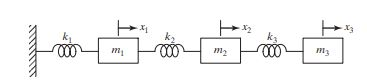
\includegraphics[scale=0.6]{15.jpg}
&	Apply&	The learner will try to \textbf{recall} the concepts of stiffness influence coefficients. &	CO 3\\
\hline
	8&	Write a short note on sweeping technique.&	Remember&	–&	CO 5\\
	\hline
	9&	Which method is most commonly used for determining fundamental frequency when the system me end in free and other end in fixed.&	Understand&	The learner will try to \textbf{recall} the various testing methods that are to be conducted  before launching  the rocket&	CO 5\\
	\hline
	10&	For solving beam problems, which numerical method is applied?&	Understand&	-&	CO 5\\
	\hline
			
		\end{longtable}
	
	\end{flushleft}
	\begin{flushleft}
		\textbf{Course Coordinator: \hspace{10cm}\textbf{HOD, AE}\\ 
			Mr. K Arun Kumar, Assistant Professor  } \\
	\end{flushleft}
\end{document}


	